\chapter{Collision Detection}
\label{chapter:collision_detection}

\textbf{Author: Fabian Kleinrad} 

This chapter is going to concern itself with the method of detecting collisions within the path planning phase. The needed information about the environment stems from the data structures covered in chapter \ref{chapter:abstract_env}. 

\section{Fundamental Principle}
An essential part of autonomy in robotics is the aspect of collision avoidance. This is only possible if the robot has the means to identify and detect possible collisions and act suitably to circumvent collisions from happening.\newline
In Autumn this step of collision detection happens alongside with path planning. With the collision detection being a very cost intensive process it is important to optimize the algorithm for better performance, while simultaneously keeping a safety margin. This safety margin is especially important since the algorithm controls an UAV. 

\subsection{Base Algorithm}
The principle of the collision detection is very simple, due to the organized and semi organized data structures the algorithm works with. To check for collisions a function can be called that takes Cartesian coordinates as parameters and returns a value that indicates if an obstacle is present or not. All the collision detection algorithm has to do is to check if there are any collisions between two points sampled by the path planning algorithm. In order two accomplish this task the Bresenham's Algorithm will be used.\newline

\subsubsection{Bresenham's Algorithm} 
The Bresenham's Algorithm is a solution to the problem of rasterizing curves. Rasterizing being the process of converting a curves or lines into cells on a grid, representing the same shape. The Algorithm covers many different shapes, but because of the nature of the path planning algorithm used only a straight line will be necessary.
The algorithm works by calculating an error for each candidate cell. The formula for this error being: $e=(y-y_0)dx-(x-x_0)dy$. Hereby $x$ and $y$ are the coordinates of the cell the error is calculated for, which are being subtracted by the coordinates of the starting point. $dx$ and $dy$ are the differences between the first and last point of the line.
The error symbolizes the deviation from the original line. By calculating the errors for each cell, it is made possible to choose cells best representing the original line.\footcite{Zingl2012}

\begin{algorithm}[]
	\caption{Bresenham's Line Algorithm\footcite{Zingl2012}}
	\SetKwFunction{Fabs}{abs}
	\SetKwFunction{FUsePixel}{UsePixel}
	$dx \gets \Fabs(x_1-x_0)$\;
	$dy \gets \Fabs(y_1-y_0)$\;
	$sx \gets x_0<x_1 ? 1 : -1$\;
	$sy \gets y_0<y_1 ? 1 : -1$\;
	$error \gets dx + dy$\;
	\While{$x_0 \neq x_1$ and $y_0 \neq y_1$}{
		$\FUsePixel(x_0, y_0)$\;
		$e_2 \gets error * 2$\;
		\If{$e_2 \geq dy$}{
			$error \gets error + dy$\;
			$x_0 \gets x_0 + sx$\;
		}\If{$e_2 \leq dx$}{
			$error \gets error + dx$\;
			$y_0 \gets y_0 + sy$\;
		}
	}
\end{algorithm}

%\begin{figure}[h]
%	\centering
%	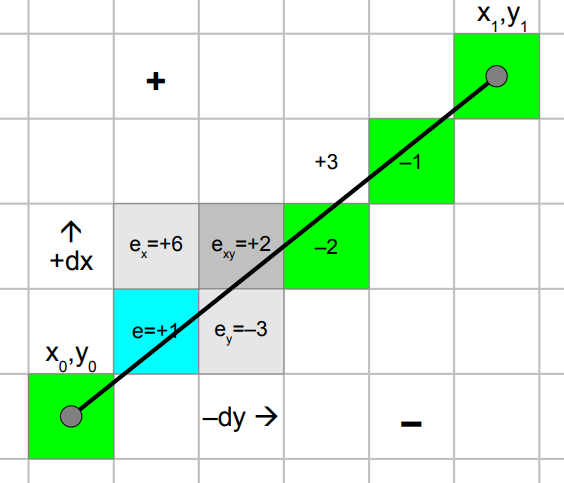
\includegraphics[width=0.5\linewidth]{img/Bresenhams}
%	\caption{Application of Bresenham's Algorithm to a straight line, %with visible errors. \cite{Zingl2012}}
%	\label{fig:collision_detection_bresenham}
%\end{figure}


\section{Implementation}
The collision detection logic is in effect every time a new point is going to be added into the graph. The path planning algorithm samples a random point and calculates its nearest neighbor. After that a function is called which takes two points and checks for collision on a straight line path between these two points.\newline
A problem that arises when using it this way is the not accounted for dimensions of the drone. For that the function takes a third parameter defining the search radius. Using that method paths can be generated suitable for the physical drone. This is accompanied by a increase in computational time. The factor of the increase amounts to $3.274r$. This stems from the way this radius, $r$, is used. For every cell that isn't the first an last cell, $2r$ neighboring cells in a line opposite to the direction of the line get checked. For the first an last cell, the radius translates to the circle where cells get checked. In order to not overlap validation areas, on the first and last cell only a semicircle is being covered. 

\begin{figure}[h]
	\centering
	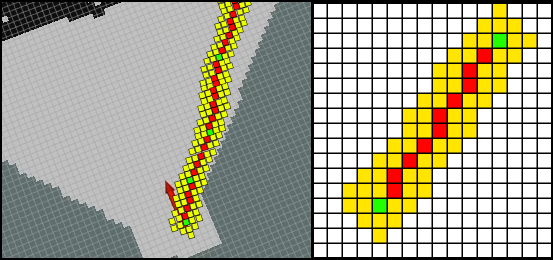
\includegraphics[width=0.8\linewidth]{img/CheckedPixels}
	\caption{Visualization of checked pixel in paths. Green being start/end points, red the lines calculated by the Bresenham's Algorithm and yellow the additionally checked cells with $r = 2$}
	\label{fig:collision_detection_checkedPixels}
\end{figure}

Therefor the to be checked cells can be calculated in dependency of the line length $l$ and radius $r$. $l$ hereby being the amount of cells present in the line calculated by the Bresenham's Algorithm. 
\[C=l+(l-2)2r+r\pi^2\]

\subsection{3 dimensional space}
When using this concept in an 3 dimensional environment, it only requires adding the new third dimension. The Bresenham's Algorithm is easy to translate into the third dimension. The problem that arises is performance. When adding the radial search, it increases the total cells checked by \(C^2 - l\).  

\section{Experiment}

In order to be able to asses the practical impact of the collision detection performed by the autumn pathfinding algorithm, an experiment was conducted, which illustrates the computational time needed, to guarantee no collisions from happening.

\subsection{Experimental Setup}

The experiment is split into two parts, these being the impact of collision detection on the computational time of two-dimensional and three-dimensional path-finding.
To get significant data, which is able to represent various scenarios in which the algorithm has to perform, a setup was selected to cover all aspects of the algorithm. The experiment works by planning a path through a static environment. This environment stays the same for all iterations of one algorithm, as well as the two different variations of the algorithm. To be able to get conclusive evidence concerning the collision detection which isn't polluted, by the random nature of the algorithm, has been set to 100. One sample refers hereby to a path planning with consistent parameters. The parameters being the amount of iterations of the RRT* algorithm($i$), the distance between the start and end node($d$), and the spacing of the nodes of the expanding tree($D$). These three parameters stay constant throughout the entire duration of the experiment, the reason being that these three Parameters affect the parts of the path planning algorithm that aren't of concern in this experiment. The Parameter controlling the behavior of the collision detection is the radius($r$).
For each radius 100 paths are being generated and each execution of the algorithm is being timed from the point of the function call till the return of the calculated path. 
The set of radii to be tested depends on the space that paths are generated in.
For each radius the mean time of all 100 data point is calculated. This results in data representing how collision detection impacts the computational time of the autumn path-planning algorithm.

\subsection{Two-dimensional Algorithm}

For autumn\_pathplanning\_2d radii starting from zero, resulting in disabling collision detection functionality, up two 2000, with a step size of 100, have been tested. 
